\chapter{Introduction}
\label{ch:introduction}


The topic of this thesis is the time propagation of semi-classical wavepackets
in special potentials which feature avoided crossings. We extend the formalism
and the algorithms to the multi-dimensional case and finally show some applications.
The work is a continuation of some earlier work \cite{FGL_semiclassical_dynamics, B_bachelor_thesis}.

In this first chapter we introduce the basic situation and the various physical
and mathematical ingredients. The main object of our studies is the time-dependent
Schrödinger equation. The Hamiltonian of the physical systems in consideration
consists of the usual kinetic operator part and a potential part. In the current
studies this potential part has a special form and models energy hypersurfaces.
We threat the fully non-adiabatic case where we allow multiple energy levels.


\section{The non-adiabatic potential}


First we introduce the potentials that are part of the Hamiltonian of our system.
In the non-adiabatic case the potential $\mat{V}$ has multiple energy levels
and the particles may switch between these surfaces. The \emph{transition probabilities}
are one of the things we are most interested in.

A potential with $N$ energy levels is given by a symmetric real-valued $N \times N$
matrix:

\begin{equation} \label{eq:potential_matrix}
  \mat{V}(\vec{x}) \assign
  \begin{pmatrix}
    v_{0,0}   & \cdots & v_{0, N-1} \\
    \vdots    & {}     & \vdots \\
    v_{N-1,0} & \cdots & v_{N-1, N-1}
  \end{pmatrix}
\end{equation}

where each entry $v_{r,c}$ is a multi-variate function depending on $\vec{x}$.
The energy levels are then given through the eigenvalues $\lambda_i(\vec{x})$
which we collect in the matrix:

\begin{equation} \label{eq:eigenlevels_matrix}
  \mat{\Lambda}(\vec{x}) \assign
  \begin{pmatrix}
    \lambda_0(\vec{x}) & {}     & {} \\
    {}                 & \ddots & {} \\
    {}                 & {}     & \lambda_{N-1}(\vec{x})
  \end{pmatrix} \,.
\end{equation}

These levels can of course intersect on a complicated subset of space. But
we are most interested in the case where they do not touch but always keep a
minimal distance between each other. This also excludes fully degenerate cases
with eigenvalues of higher multiplicity. Therefore it is possible to sort
the energy levels like:

\begin{equation}
  \lambda_0(\vec{x}) > \lambda_1(\vec{x}) > \cdots > \lambda_i(\vec{x}) > \cdots > \lambda_{N-1}(\vec{x})
\end{equation}

independently of $\vec{x}$. The situation where two energy levels come closer
to each other in a (small) region of space but do not intersect is called an
\emph{avoided crossing}. An example of a two-dimensional non-adiabatic potential
with two energy levels is shown in figure \ref{fig:conic_avoided}.

\begin{figure}
  \centering
  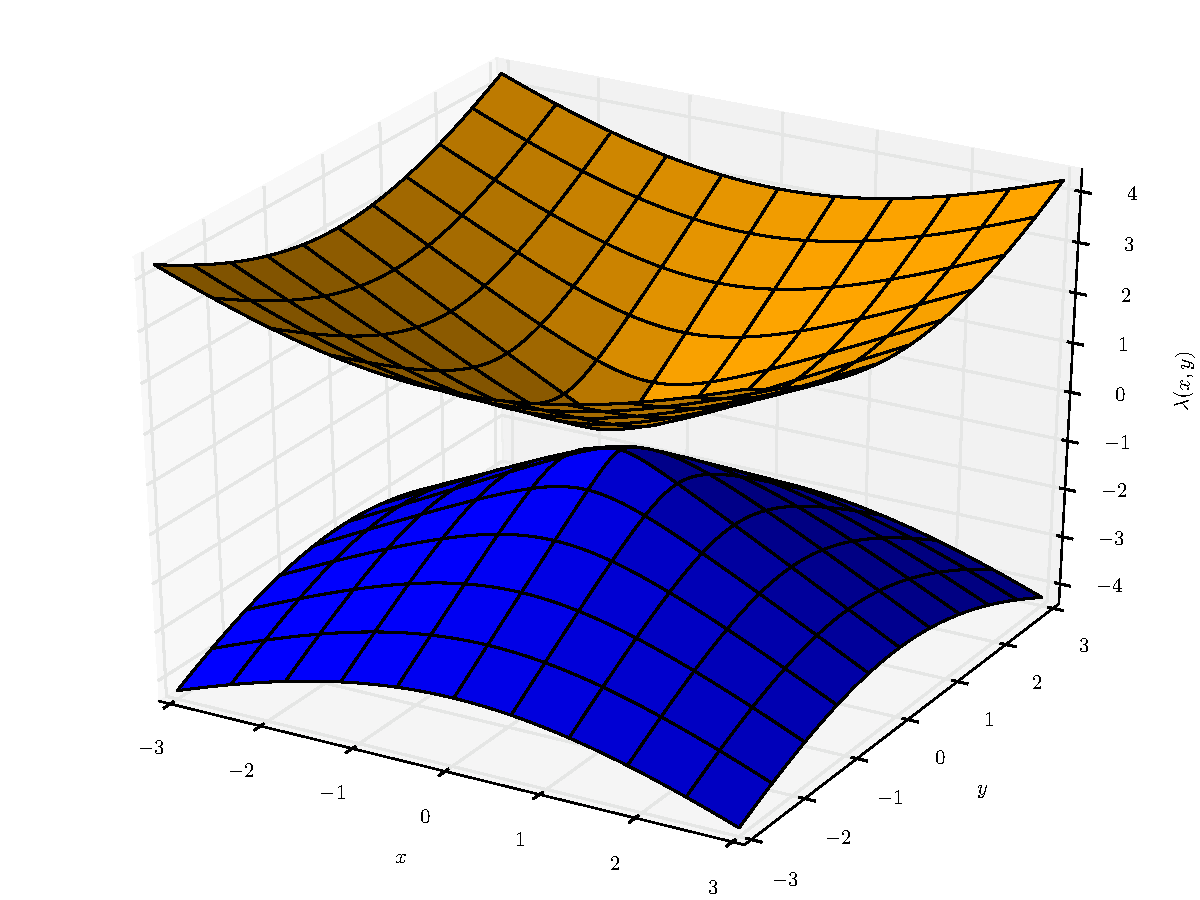
\includegraphics[width=0.7\linewidth]{./fig/conic_avoided.pdf}
  \caption[Example of an avoided crossing]
          {A two-dimensional potential having two energy levels with a conical
           avoided crossing. (Type 3 avoided crossing according to \cite{HJ_molecularpropagation}.)}
  \label{fig:conic_avoided}
\end{figure}

Given a non-adiabatic potential by its matrix $\mat{V}(\vec{x})$ the diagonalisation
process can be written as follows:

\begin{equation} \label{eq:eigentransformation}
  \mat{\Lambda}(\vec{x}) = \mat{M}\inv(\vec{x}) \mat{V}(\vec{x}) \mat{M}(\vec{x})
\end{equation}

and $\mat{\Lambda}(\vec{x})$ is the diagonalised version containing the different
energy levels $\lambda_i(\vec{x})$. This is often called the adiabatic basis,
exhibiting no coupling between the energy levels $\lambda_i(\vec{x})$.
The linear transformation is then given by the matrix:

\begin{equation} \label{eq:eigentransformation_matrix}
  \mat{M}(\vec{x}) \assign
  \begin{pmatrix}
    \vdots         &        & \vdots \\
    \nu_0(\vec{x}) & \cdots & \nu_{N-1}(\vec{x}) \\
    \vdots         &        & \vdots
  \end{pmatrix}
\end{equation}

where we stacked the eigenvectors $\nu_{i}$ as columns. We will need this
eigentransformation later during the computation of observables.


\section{The wavefunction}


The next objects we introduce are \emph{wavefunctions} which are omnipresent in
quantum physics and chemistry. We work in $D$ space dimensions of flat Euclidean space.
Let $x_0, x_1, \ldots, x_{D-1}$ denote the basis directions and $\vec{x} \in \mathbb{R}^D$
be an arbitrary point in this space.

The wavefunction $\psi$ depends on position $\vec{x}$ and time $t$. Formally
we define the wavefunction to be:

\begin{equation} \label{eq:wavefunction}
\begin{split}
  \psi : \mathbb{R}^D \times \mathbb{R} & \rightarrow \mathbb{C} \\
         \left(\vec{x}, t\right)        & \mapsto     \psi\left(\vec{x}, t\right) = z
\end{split}
\end{equation}

and use the following Dirac braket notation:

\begin{equation}
  \Ket{\psi} \assign \psi\left(\vec{x}, t\right) = \psi\left(x_0, \ldots, x_{D-1}, t\right) \,.
\end{equation}

Often we will omit the explicit time dependence and consider only a static
picture at a fixed time $t_0$ where the wavefunction is given as:

\begin{equation}
\begin{split}
  \psi : \mathbb{R}^D & \rightarrow \mathbb{C} \\
         \vec{x}      & \mapsto     \psi(\vec{x}) = z \,.
\end{split}
\end{equation}

For performing simulations within non-adiabatic potentials we need compatible
wavefunctions. In our case this implies that the wavefunction must have $N$
components:

\begin{equation}
  \psi \assign
  \begin{pmatrix}
    \psi_0 \\
    \vdots \\
    \psi_{N-1}
  \end{pmatrix}
\end{equation}

with each component $\psi_i$ complying with \eqref{eq:wavefunction}. Such a
wavefunction is appropriate for a $N$-level potential. After an eigentransformation
we can interpret each $\psi_i$ as the probability distribution on the energy level
$\lambda_i$.


\section{The time-dependent Schrödinger equation}


The next subject to look at is the time-dependent Schrödinger equation.
It is the governing equation for all time-dependent quantum mechanical
phenomena. This equation describes the time evolution of a wavefunction.
The partial differential equation can be written as:

\begin{equation} \label{eq:basics_tdse_simple}
  i \hbar \frac{\partial}{\partial t} \Ket{\psi} = H \Ket{\psi}
\end{equation}

where $H$ denotes the Hamiltonian operator and $\hbar$ is the Planck constant.
However we do not use this version directly but study a rescaled version.
What we use is the so-called \emph{semi-classical scaling} of the Schrödinger
equation. Instead of $\hbar$ we introduce a real-valued parameter consistently
denoted by $\varepsilon$ which is strictly positive
\footnote{Other authors use $\varepsilon$ or even $\hbar$ (without its physical
meaning and value) for the quantity we denote by $\varepsilon^2$.}.
This parameter usually takes values in the range of about $0.001$ up to $0.1$.
It is worthwhile to note that in the limit $\varepsilon \rightarrow 0$ we
are back in the classical world and for bigger $\varepsilon$ we get more and more
quantum effects.

The rescaled Schrödinger equation still keeps its mathematical form and looks
like:

\begin{equation} \label{eq:basics_tdse_semi}
  i \varepsilon^2 \frac{\partial}{\partial t} \Ket{\psi} = H \Ket{\psi} \,.
\end{equation}

The Hamiltonian operator is given by:

\begin{equation}
  H \assign T + V(\vec{x})
\end{equation}

where we obtain the kinetic operator $T$ by the correspondence principle from
classical mechanics. Start with the definition of the kinetic energy:

\begin{equation*}
  T \assign \frac{\vec{p}\cdot\vec{p}}{2m}
\end{equation*}

and set the mass $m=1$ (absorb it into the scaling parameter). In one dimension
the momentum operator is:

\begin{equation*}
  p \assign -i \varepsilon^2 \pdiff{}{x}
\end{equation*}

and we find that:

\begin{equation*}
  T \assign - \frac{\varepsilon^4}{2} \pdiff[2]{}{x} \,.
\end{equation*}

In higher dimensions we have:

\begin{equation*}
  p_{i} \assign -i \varepsilon^2 \pdiff[2]{}{x_i}
\end{equation*}

and in turn:

\begin{equation} \label{eq:kinetic_operator_scalar}
  T \assign - \frac{\varepsilon^4}{2} \Delta
\end{equation}

for the quantum mechanical equivalent.

In case of non-adiabatic potentials the Schrödinger equation becomes vector-valued
and instead of \eqref{eq:basics_tdse_semi} we should write:

\begin{equation} \label{eq:basics_tdse_vector}
  i \varepsilon^2 \frac{\partial}{\partial t} \Ket{ \begin{pmatrix}
                                                   \psi_0 \\
                                                   \vdots \\
                                                   \psi_{N-1}
                                                 \end{pmatrix}
                                               }
  =
  \begin{pmatrix}
    {} & {}       & {} \\
    {} & \mat{H}  & {} \\
    {} & {}       & {}
  \end{pmatrix}
  \Ket{ \begin{pmatrix}
          \psi_0 \\
          \vdots \\
          \psi_{N-1}
        \end{pmatrix} } \,.
\end{equation}

The Hamiltonian operator is matrix-valued now:

\begin{equation}
  \mat{H} \assign \mat{T} + \mat{V}(\vec{x}) \,.
\end{equation}

The kinetic operator $\mat{T}$ is block-diagonal with each entry being of
the form shown in \eqref{eq:kinetic_operator_scalar}.

We can solve the Schrödinger equation by a separation of variables ansatz and
find the following result for the time propagation of any quantum state $\Ket{\psi\ofs{t}}$:

\begin{equation} \label{eq:basics_analytic_time_propagation}
  \Ket{\psi\ofs{t}} = \exp\left(- \frac{i}{\varepsilon^2} \mat{H} t \right) \Ket{\psi\ofs{0}} \,.
\end{equation}

However we can almost never compute the exponential of $\mat{H}$ in closed form.
In the remaining chapters of this thesis we try to solve this equation by
superior numerical methods.
